\chapter{Method}
In this chapter the work environment and the procedure is explained. 

\section{Frameworks and tools}
This work uses Python $3.8.10$ as programming language for the data analysis as well as for the training and evaluation of the models. Python already offers many high-end libraries for \gls{ml}. Jupyter notebooks were used to write and adjust all code. Important snippets were moved into python files to reuse it in multiple notebooks.

\section{Public plant disease datasets}
\label{section:plant_datasets}

There are several datasets on plant diseases publicly available, but only a few meet the requirements such as sufficient size and appropriate image resolution. The following Table \ref{tab:suitable_plant_datasets} lists the suitable plant disease datasets used in this work. The complete list regarded plant datasets including links is in the Appendix \ref{appendix:datasets_tables}.

%TODO add citation to PlantDataset
\begin{table}[H]
\centering
\caption{Large plant disease datasets \label{tab:suitable_plant_datasets}}
\begin{tabularx}{\textwidth}{|
 >{\hsize=.72\hsize}X |
 >{\hsize=.14\hsize\raggedleft}X |
 >{\hsize=.14\hsize\raggedleft}X |
}
\hline
\textbf{Name} & \textbf{\#Images} & \textbf{\#Classes} \tabularnewline \hline
PlantVillage Dataset (PVD) \autocite{hughes2016} & 54'303 & 38 \tabularnewline \hline
Cassava Leaf Disease Classification \autocite{mwebaze2020} & 21'398 & 5 \tabularnewline \hline
PlantDataset \autocite{pal2022} & 5'106 & 20 \tabularnewline \hline
PlantDoc \autocite{singh2020} & 2'598 & 28 \tabularnewline \hline
DARMA \autocite{keaton2021} & 231'414  & 1'000 \tabularnewline \hline
Plant Disease Diagnosis Dataset (PDDD) \autocite{dong2023} & 421'133  & 120 \tabularnewline \hline
\end{tabularx}
\end{table}

All datasets were checked for obvious duplicates and cleaned up if necessary. \autocite{groeger2023} shows, that some of the datasets also have label errors and near duplicates with different magnifications or similar small changes. These changes make it harder to detect such cases. For the sake of simplicity the duplicate check in this work only covers images with the exact same image hash or the same file name combined with manual verification. The complete list of cleaning steps is in the Appendix \ref{appendix:data_quality_assessment}.

\subsection{PlantVillage Dataset (PVD)}
All images in the dataset have a lab-controlled background as shown in Figure \ref{fig:example_images_of_plantvillage}.

\begin{figure}[H]
    \begin{center}
    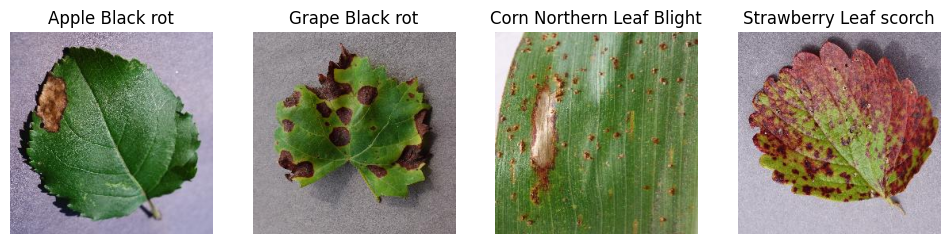
\includegraphics[width=15cm]{../images/example_images_of_plantvillage.png}
    \caption{Example images of PlantVillage}
    \label{fig:example_images_of_plantvillage}
    \end{center}
\end{figure}

This dataset does not provide a split for a test test. Therefore, the splitting was carried out by myself using 80\% of the data for the training set and 10\% each for the validation and test set. The stratifying ensures, that the distribution of the 38 classes is the same over all sets, which can be seen in Figure \ref{fig:class_distribution_of_plantvillage}. 
% Without a given split is also not possible to have a meaningful line.

\begin{figure}[H]
    \begin{center}
    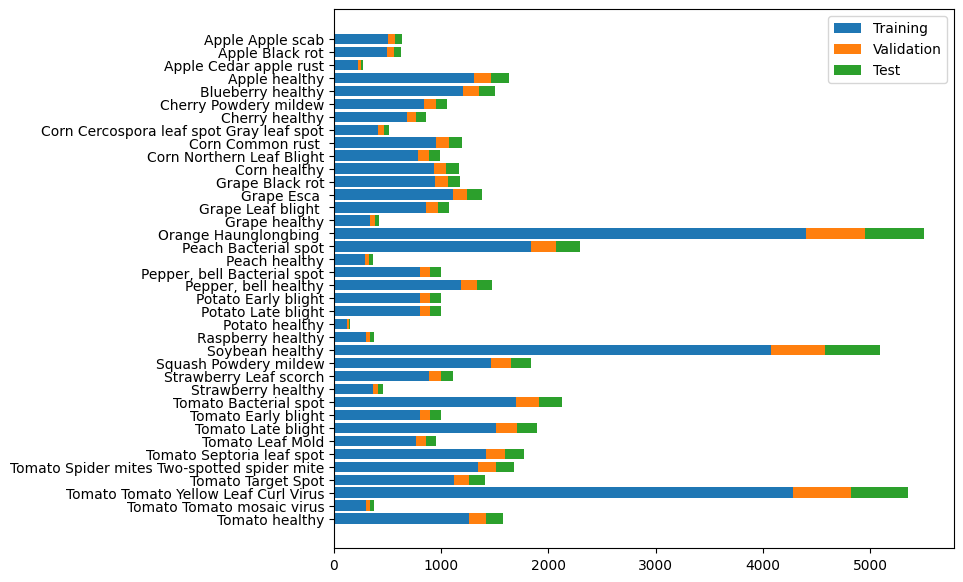
\includegraphics[width=15cm]{../images/class_distribution_of_plantvillage.png}
    \caption{Class distribution of PlantVillage}
    \label{fig:class_distribution_of_plantvillage}
    \end{center}
\end{figure}

\subsection{Cassava Leaf Disease Classification}
Figure \ref{fig:example_images_of_cassava}.

\begin{figure}[H]
    \begin{center}
    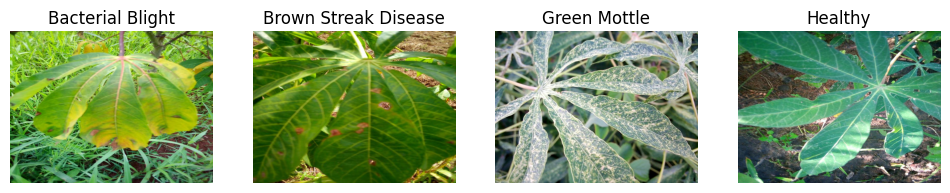
\includegraphics[width=15cm]{../images/example_images_of_cassava.png}
    \caption{Example images of Cassava}
    \label{fig:example_images_of_cassava}
    \end{center}
\end{figure}

Figure \ref{fig:class_distribution_of_cassava}

\begin{figure}[H]
    \begin{center}
    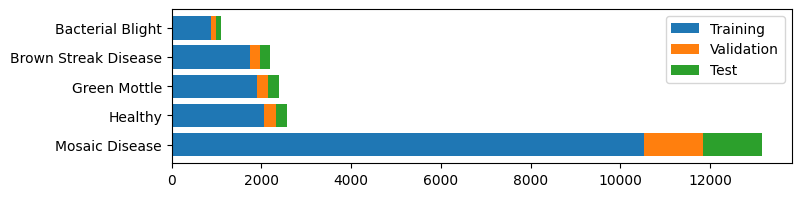
\includegraphics[width=15cm]{../images/class_distribution_of_cassava.png}
    \caption{Class distribution of Cassava}
    \label{fig:class_distribution_of_cassava}
    \end{center}
\end{figure}


\subsection{PlantDataset}
\subsection{PlantDoc}
\subsection{DARMA}
\subsection{Plant Disease Diagnosis Dataset (PDDD)}

\section{Models}
